%\newcommand{\Exp}{\mathbb{E}}

% reset section counter
\setcounter{section}{0}

%\metadata{lecture ID}{Your names}{date}
\metadata{4}{Jack Collison}{April 23, 2021}
\sec{Review and overview}

In the previous lecture, we delved into local polynomial regressions, cross validation, hyperparameter tuning, and an introduction to splines. In particular we talked about cubic splines and natural cubic splines. 

In this lecture, we will continue our discussion on natural cubic splines in more depth. We will also talk about nearest-neighbor methods, challenges in high-dimensional nonparametrics, and the kernel method.
\sec{Splines}

Let's quickly review splines from our previous lecture. The basic principle of a spline is to minimize a regularized objective function over function $\hat{r}$ to some data $\{(x_i, Y_i) : 1 \leq i \leq n\}$

\begin{equation}
    L_\lambda(\hat{r}) \triangleq \argmin_{\hat{r}} \sum_{i=1}^n \left( Y_i - \hat{r}(x_i) \right)^2 + \lambda \int \hat{r}''(x)^2dx ,
\end{equation}
where the regularization term $\lambda \int \hat{r}''(x)^2dx$ encourages $\hat{r}$ to be as smooth as possible. Here, ``smooth'' means the second order derivative is as small as possible (i.e. we want a very small regularization penalty). 

\subsec{A brief review}
Let's recall a few important theorems and lemmas. From the last lecture, we know that the minimizer $\hat{r}$ of this objective function is a natural cubic spline.

\begin{theorem}
    The minimizer $L_\lambda(\hat{r})$ is a natural cubic spline with $n$ knots at data points $\{x_i : 1 \leq i \leq n\}$. That is, $\hat{r}$ must be a cubic spline.
\end{theorem}
A natural cubic spline is a piecewise polynomial function that linearly extrapolates near $\pm \infty$. Let's also recall an important lemma from last time.

\begin{lemma}
    A cubic spline with knots $\xi_1, ..., \xi_n$ forms a $(n + 4)$-dimensional subspace of functions. That is, there exist some $\{h_j : 1 \leq j \leq n+4\}$ such that the cubic spline $\hat{r}$ can be written as
    \begin{equation*}
        \hat{r} = \sum_{j=1}^{n+4} \beta_j h_j(x),
    \end{equation*}
    where $\beta_j \in \mathbb{R}$ for $j=1,\cdots, n+4$.
\end{lemma}
Now, we have a strong structural form in the cubic spline and only have to search over a finite dimensional subspace in the functional form specified above. We can use this functional form of $\hat{r}$ in our penalized regression from above.

\begin{equation*}
    L_\lambda(\hat{r}) = L_\lambda(\beta) = \sum_{i=1}^n \left( Y_i - \sum_{j=1}^{n+4} \beta_j h_j(x_i) \right)^2 + \lambda \int \left( \sum_{j=1}^{n+4} \beta_j h_j''(x_i)\right)^2dx.
\end{equation*}
Although this looks like a complex objective function, we have a finite number of parameters $\{\beta_j : 1 \leq j \leq n + 4\}$ to optimize over. Further, $L_\lambda(\beta)$ is a convex quadratic function in $\beta$. We can see this by expanding out the squared terms. As $\beta$ is not a function of $x$, the $\beta_j$'s in the regularization term will be unaffected by the derivatives. This makes it a much more feasible problem and allows us to write it in matrix form.

\subsec{Matrix notation for splines}
Although we have a convex quadratic functional form, the problem remains notationally burdensome. Let's continue by translating our optimization problem into matrix notation. First, let's define a few matricies that will be useful later.

\begin{equation}
    F = \begin{bmatrix} 
             h_1(x_1) & ... & h_{n+4}(x_1) \\ 
             & ... & \\
             h_{1}(x_n) & ... & h_{n+4}(x_n)
        \end{bmatrix} \in \mathbb{R}^{n \times (n+4)}, \qquad
    \beta = \begin{bmatrix} \beta_1 \\ ... \\ \beta_{n+4} \end{bmatrix} \in \mathbb{R}^{n+4}, \qquad 
    Y = \begin{bmatrix} Y_1 \\ ... \\ Y_n \end{bmatrix} \in \mathbb{R}^{n}.
\end{equation}
Applying matrix multiplication in lieu of our summations before, we find
\begin{equation*}
    Y - F \beta = \begin{bmatrix} Y_1 \\ ... \\ Y_n \end{bmatrix} - \begin{bmatrix} \beta_1h_1(x_1) + ... + \beta_{n+4}h_{n+4}(x_1) \\ ... \\ \beta_1h_1(x_n) + ... + \beta_{n+4}h_{n+4}(x_n) \end{bmatrix},
\end{equation*}
and therefore
\begin{equation*}
    \sum_{i=1}^n \left(Y_i - \sum_{j=1}^{n+4} \beta_jh_j(X_i)\right)^2 = ||Y - F\beta||_2^2.
\end{equation*}
Then we look at the regularization term, since
\begin{align*}
    \int \left( \sum_{j=1}^{n+4} \beta_jh_j''(x) \right)^2dx & = \int \left( \sum_{j=1}^{n+4} \sum_{k=1}^{n+4} \beta_j\beta_k h_j''(x) h_k''(x) \right)dx \\
    &= \sum_{j=1}^{n+4}\sum_{k=1}^{n+4} \beta_j\beta_k \left( \int h_j''(x)h_k''(x)dx \right),
\end{align*}
by defining the term $\Omega_{jk}$ as
\begin{equation*}
    \Omega_{jk} \triangleq \int h_j''(x)h_k''(x)dx,
\end{equation*}
we have $\Omega = [\Omega_{jk}] \in \mathbb{R}^{(n+4)\times(n+4)}$ and
\begin{equation*}
    \sum_{j=1}^{n+4}\sum_{k=1}^{n+4} \beta_j\beta_k \left( \int h_j''(x)h_k''(x)dx \right) = \sum_{j=1}^{n+4}\sum_{k=1}^{n+4} \beta_j\beta_k\Omega_{jk} = \beta^\top \Omega \beta.
\end{equation*}
Now that we have translated each part of the objective function, we can finally write it as
\begin{equation*}
    L_\lambda(\beta) \triangleq ||Y - F\beta||_2^2 + \lambda \beta^\top \Omega \beta.
\end{equation*}
This is a remarkably familiar functional form which reminds us of a simple linear regression and ridge regression. The regularization is weighted by matrix $\Omega$. In the case that we have $\Omega = I$, then we have

$$\beta^\top \Omega \beta = \beta^\top \beta = ||\beta||_2^2,$$
which is exactly a ridge penalty.
\subsec{Minimizing the regularized objective}
Given its similarities to linear regression, we can solve this objective function analytically in a similar fashion to that. That is, we will compute the gradient
\begin{equation*}
    \nabla L_\lambda(\beta) = -2F^\top (Y - F\beta) + 2\lambda \Omega\beta,
\end{equation*}
and set it equal to zero. Solving the above linear equation, we find
\begin{equation*}
    \hat\beta = (F^\top F + \lambda\Omega)^{-1} F^\top Y.
\end{equation*}
And therefore the minimizing natural cubic spline is then
\begin{equation*}
    \hat{r}(x) = \sum_{j=1}^{n+4} \hat\beta_jh_j(x). 
\end{equation*}
\subsec{Choosing the basis}
Now that we have analytically solved for $\hat{r}$, we might wonder how to choose $h_1, ..., h_{n+4}$. In the last lecture, we saw an example of a basis given by $h_{i+4} = (x - \xi_i)_+^3$ where $\xi_i$ is a knot in our spline. When choosing a basis, we should always remember that we must derive $\Omega$ which requires integration. Therefore, our choice of basis should be relatively easy to integrate. Of course, this can be done numerically but it's a much simpler problem when we are able to integrate and know properties of the basis (i.e. to speed up computation of $F^\top F$ in our estimate of $\beta$). 

The textbook refers to $B$-splines as a good basis for computational reasons and because they have nice properties. We will not delve into this here.
\sec{Interpretation of splines}

\subsec{Splines as linear smoothers}

First, let's recall that a linear smoother is a family of functions that takes an average of the response variable (i.e. our $Y$ variable). Splines fall within this family of linear smoothers. We will show why this is true. Let's begin by recalling our definition of $\hat\beta$ and $\hat{r}$.
\begin{equation*}
    \hat\beta = (F^\top F + \lambda\Omega)^{-1} F^\top Y, \qquad \hat{r}(x) = \sum_{j=1}^{n+4} \hat\beta_jh_j(x).
\end{equation*}
By taking $h(x) = \begin{bmatrix} h_1(x) & \cdots & h_{n+1}(x) \end{bmatrix}^\top \in \mathbb{R}^{n+4}$, we can write
\begin{align*}
	\hat{r}(x) & = h(x)^\top  (F^\top F + \lambda\Omega)^{-1} F^\top Y := LY,
\end{align*}
where $L = h(x)^\top  (F^\top F + \lambda\Omega)^{-1} F^\top$, meaning our spline is indeed a linear smoother, as required. It is important to show that this falls into the family of linear smoothers because it means that we can apply our methods of cross validation (which were defined for linear smoothers) to splines as well.
\subsec{Splines approximated by kernel estimation}

In general, splines and local linear regression will perform approximately equivalently. It will be hard to find consistent cases where one outperforms the other; it simply depends on the noise in the data. Let's quickly recall the kernel estimator:
$$
\hat{r} = \frac{\sum_{j=1}^n w_jY_j}{\sum_{j=1}^n w_j}, \qquad w_j = K\left( \frac{x_j - x}{h} \right).
$$
Note that $K$ is our kernel function (e.g. Gaussian, boxcar, etc.). Splines approximately correspond to a similar functional form.
$$
\hat{r} \approx \frac{\sum_{j=1}^n w_jY_j}{\sum_{j=1}^n w_j}, \qquad w_j = \frac{n^{\frac{1}{4}}}{\lambda^{\frac{1}{4}}f(x)^{\frac{3}{4}}} K\left( \frac{x_j - x}{ \left( \frac{\lambda}{nf(x_j)} \right)^{\frac{1}{4}}} \right).
$$
This is clearly much more complicated that our standard kernel estimator for a number of reasons. First, we can notice that we have a dependency on the density $f(x)$ of $x$. Next, our kernel $K$ is typically not the Gaussian kernel (although it is usually something relatively reasonable). Finally, we have a bandwidth that depends on $f(x)$. 

Therefore, splines can be considered a special form of local averaging. They have the advantage in that they tend to better fit the global structure of the data due to the ``global'' penalization term that encourages smoothness.
\subsec{Advanced spline methods}
There exist more advanced spline methods, although we won't dive too deeply into them here. For example, there is a method that has knots that aren't necessarily on data points. In our penalized regression above, we mandated that the knots fell onto a data point in order to properly penalize the objective function. Other methods do not have this requirement. Other methods also allow us to fix knots $q_1, ..., q_m$ in advance while still others put knots in the optimization problem (i.e. the function also optimizes over the placement of knots and chooses their locations).
\subsec{Confidence bands}
Confidence intervals (or bands) are always important in statistics. We want to know how close we are to the ground truth functional form of the data and we want to know where our estimates might be more different from the ground truth (i.e. we want a more interpretable estimate).
\begin{figure}[htbp!]
	\centering
    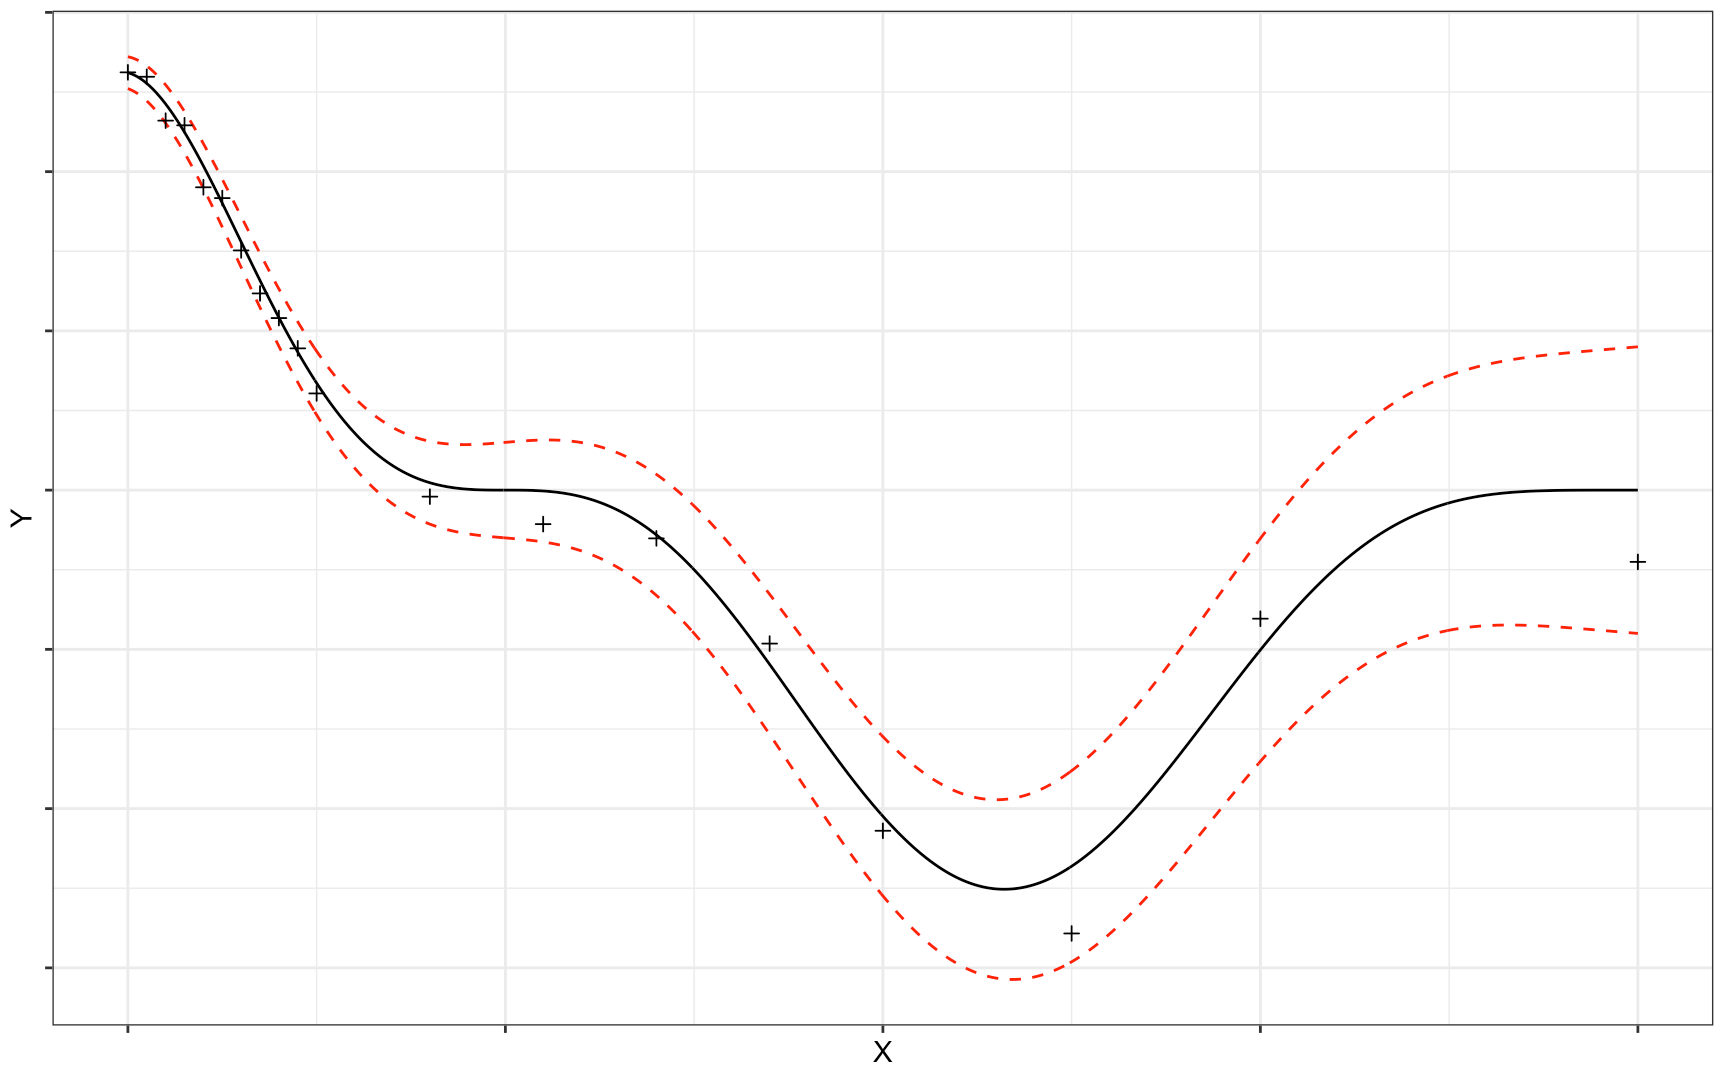
\includegraphics[scale = .4]{figure/Lecture04/graph.png}
    \caption{A example of spline along with its confidence band.}
\end{figure}
Our confidence band will be of the typical form
$$
[\hat{r} - \hat{s}(x), \hat{r} + \hat{s}].
$$
In the case of splines, we have an estimate of $\hat{r}(x)$ and wish to find the standard deviation of $\hat{r}(x)$ defined as $\hat{s}(x)$. That is, we want to find a confidence band around our estimates that contains the true function $r(x)$. In practice, this is difficult since we do not know the difference between $\mathbb{E}[\hat{r}(x)]$ and $r(x)$. Statisticians thus find the confidence band for $\mathbb{E}[\hat{r}(x)]$. For this purpose, we find $\hat{s}(x) \approx \text{SD}(\hat{r}(x))$. 

We can do this for the general family of linear smoothers with the general form
$$
\hat{r}(x) = \sum_{i=1}^n l_i(x)Y_i.
$$
From here, we can find the variance of $\hat{r}(x)$.
\begin{align*}
    \text{Var}(\hat{r}(x)) &= \text{Var}\left( \sum_{i=1}^n l_i(x)Y_i \right) \sum_{i=1}^n l_i(x)^2 \text{Var}(Y_i) = \sum_{i=1}^n l_i(x)^2 \sigma^2 = \sigma^2 ||l(x)||_2^2.
\end{align*}

\noindent Notice that we assume $\text{Var}(Y_i) = \sigma^2$ for each $\{(Y_i) : 1 \leq i \leq n\}$ and define $l(x) = \begin{bmatrix} l_1(x) \\ .... \\ l_n(x) \end{bmatrix}$. Thus, our confidence band becomes
$$
[\hat{r} - c \cdot \sigma \cdot ||l(x)||_2, \hat{r} + c \cdot \sigma \cdot ||l(x)||_2].
$$

\noindent Notice the addition of the variable $c$ which is chosen based on the level of confidence desired. A large value of $c$ will have higher confidence whereas a small value of $c$ will have lower confidence.

\sec{Nonparametrics in high dimension}
In order to motivate this discussion of high dimensional statistics, we will begin by examining our toolbox of nonparametric techniques in the context of higher dimensional data. Let's consider the case when we have $X \in \mathbb{R}^d$ where $d > 1$. 

There are some immediate challenges to local averaging, including the construction of neighborhoods. A natural first thought would be to construct a ``sphere'' $B_x = \{x' : ||x' - x||_2 \leq h\}$ around some fixed point $x$. This is a problem in high dimensions because the distance between points often is not informative. They are often far away from one another in high dimensions.

\subsec{Examples}

\begin{example}
Suppose we generate $x^{(1)}, ..., x^{(n)} \iid \text{Unif}(s^{d-1})$ where the superscripts denote the index of the data points and $s^{d-1}$ is a $d$-dimensional unit sphere defined as $\{x : ||x||_2 = 1, x \in \mathbb{R}^d\}$. 
\end{example}
In this case, with $p \geq 1 - n^2\text{exp}(-\Omega(d))$, we have
$$
\forall i, j \in [n], ||x^{(i)} - x^{(j)}||_2 \approx \sqrt{2} \Rightarrow \langle x^{(i)}, x^{(j)} \rangle \approx 0.
$$
This is problematic because the distance between points isn't that big since each $x$ is orthogonal to all other values of $x$. The distance isn't informative in this case. That is, if we take $h \gg \sqrt{2}$, then we have all data points in our neighborhood. However, if we take $h \ll \sqrt{2}$, then we have no points in our neighborhood.

\begin{example}
Let's consider the example of comparing images as in Fig.~\ref{fig:fig2}.
\begin{figure}
	\centering
    
\includegraphics[scale = .4]{figure/Lecture04/image_flip.png}
	\caption{Example of image comparison.} \label{fig:fig2}
\end{figure}
\end{example}
The distances between these two images will appear as very large just comparing the pixels, even if they are closely related.

\subsec{$k$-Nearest neighbors algorithm}

\noindent One of the most prominent algorithms for high dimensional data is the $k$-nearest neighbors method. Before diving into this algorithm, we must first note that it doesn't always solve a problem, but will potentially make it easier to handle. The algorithm is defined as follows.
\begin{enumerate}
    \item $\forall x$, let $B_x = \{i : x^{(i)} \text{ is among the } k \text{ closest neighbors of } x\}$;
    \item $\hat{r}(x) = \frac{1}{k} \sum_{i \in B_x} Y_i$.
\end{enumerate}
A benefit of this algorithm is that each bin $B_x$ will always contain $k$ points, so we don't need to worry about bandwidth. Of course, this doesn't always alleviate the problem that the neighbors might not be meaningful (i.e. they could be neighbors just by chance). The plots in Fig.~\ref{fig:fig3} explore a few different values for $k$ on a toy dataset ($k \in \{10, 50, 400\}$).

\begin{figure}
	\centering
	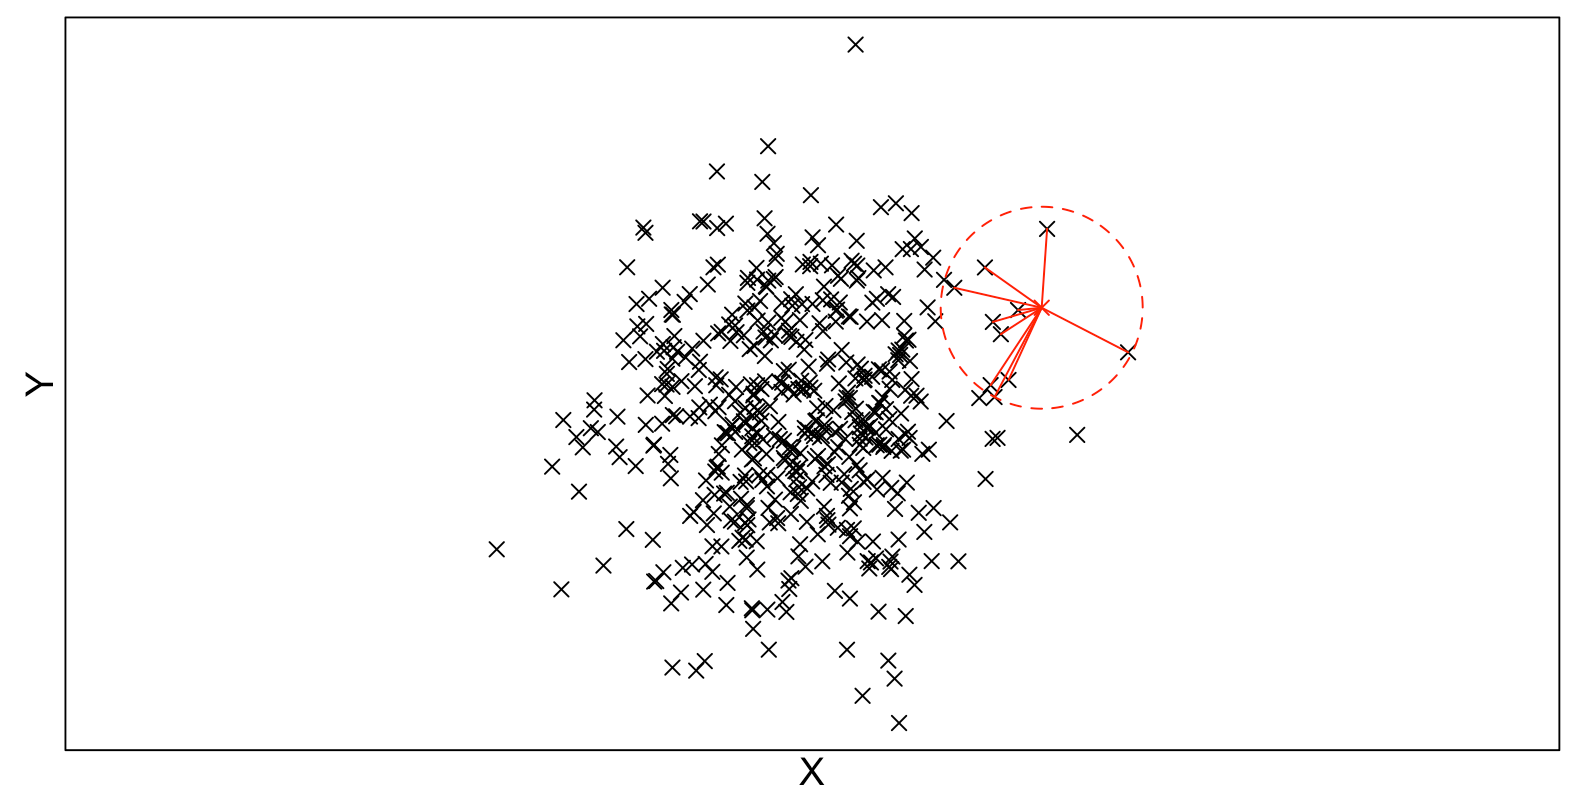
\includegraphics[scale = .18]{figure/Lecture04/knn10.png}
	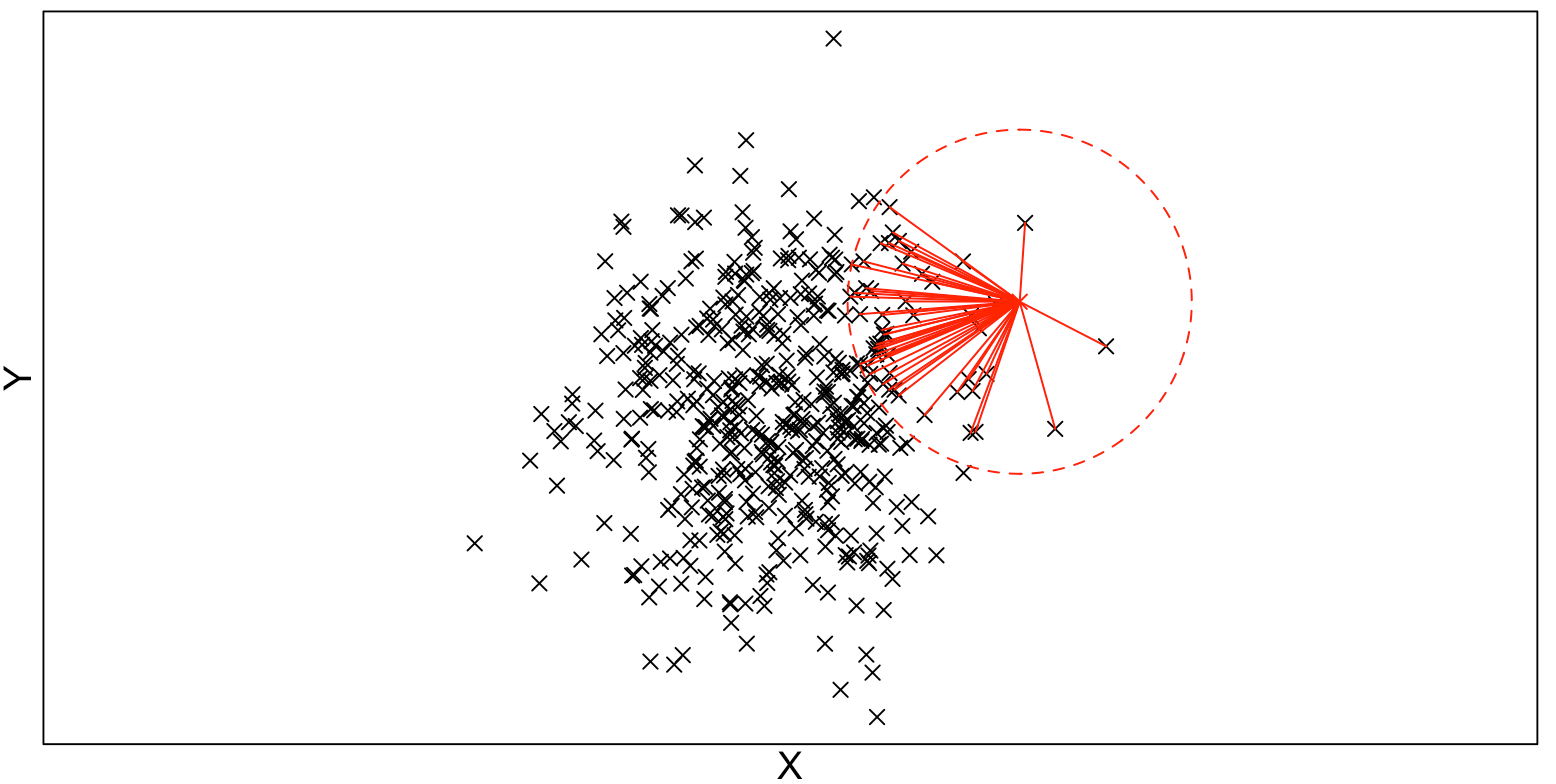
\includegraphics[scale = .18]{figure/Lecture04/knn50.png}
	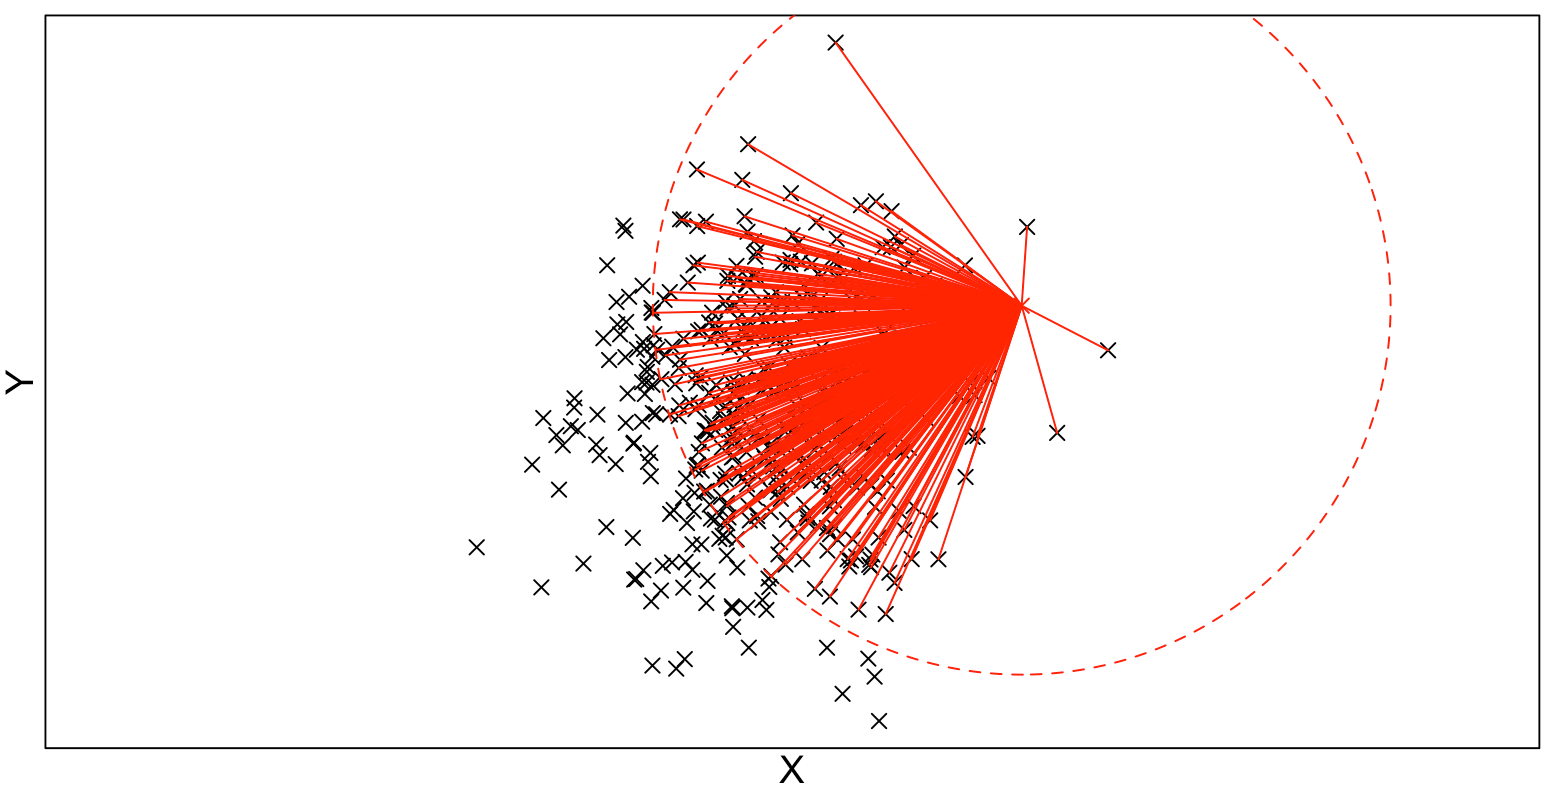
\includegraphics[scale = .18]{figure/Lecture04/knn400.png}
	\caption{Examples of $k$-NN with $k=10$ (Left), $k=50$ (Middle) and $k=400$ (Right).} \label{fig:fig3}
\end{figure}

However, there is the fundamental limitation in the curse of dimensionality. That is, nonparametric methods require a sample size exponential in dimension $d$. A bit more formally, if we only assume Lipschitzness or smoothness conditions (e.g. $||r(x) - r(x')|| \leq ||x - x'||$ or bounds on second order derivatives) then any estimator of $\hat{r}$ will have errors on the order of $n^{-\frac{1}{\Omega(d)}}$. That is, we have
$$
\epsilon = n^{-\frac{1}{\Omega(d)}} \Rightarrow n \geq \left( \frac{1}{\epsilon} \right)^{\Omega(d)}.
$$

\sec{Kernel method}

\noindent We will now explore the kernel method (not to be confused with our previous kernel estimators). In order to begin, let's introduce some notation. Our training dataset is defined as
$$
\left(x^{(1)}, y^{(1)}\right), ..., \left(x^{(n)}, y^{(n)}\right), \qquad x^{(i)} \in \mathbb{R}^d, y^{(i)} \in \mathbb{R}.
$$
The general idea of the kernel method is to generate a feature map defined as 
$$
\phi : x \in \mathbb{R}^d \rightarrow \phi(x) \in \mathbb{R}^m,
$$
where $x \in \mathbb{R}^d$ are our input and $\phi(x) \in \mathbb{R}^m$ are our features. Note that $m$ can be very big or even infinite. More specifically, we want to transform our standard database into a different feature-space.
$$
\left\{ \left( x^{(i)}, y^{(i)} \right) \right\}_{i=1}^n \rightarrow \left\{ \left( \phi \left( x^{(i)} \right), y^{(i)} \right) \right\}_{i=1}^n.
$$
After converting this to a higher dimension, we can run a standard parameterized method on the transformed dataset (e.g. a linear regression).

\subsec{Motivating examples}

\begin{example}
	Let's consider nearest neighbors with $\ell_2$ distance in the feature space. That is, we have $d(x, z) = ||\phi(x) - \phi(z)||_2^2$. If we design $\phi(\cdot)$ in the right way, our distance metric $d(\cdot, \cdot)$ will be more informative than the typical $||x - z||_2^2$. For example, applying $\phi$ could make transformed values $\phi(x)$ and $\phi(z)$ closer than their untransformed counterparts.
\end{example} 
\begin{example}
	We can apply the same logic to traditional linear models. That is, we can apply $\phi(x)$ and fit a linear model to the transformed data to extract more signal. Suppose we have $x, y \in \mathbb{R}$ with linear model $y = \theta_0 + \theta_1 x$. Now, let's say $\phi(x) = (1, x, x^2, x^3) \in \mathbb{R}^4$. We can then fit a linear regression on top of this transformed data
	$$
	y = \theta^\top \phi(x) = \begin{bmatrix} \theta_0 \\ \theta_1 \\ \theta_2 \\ \theta_3 \end{bmatrix}\phi(x) = \theta_0 + \theta_1x + \theta_2x^3 + \theta_3x^3.
	$$
	This is a more flexible polynomial model that can be expanded even beyond the third degree to represent any polynomial. This allows us to rely less on the assumptions of linear regression by transforming our input into a higher dimension.
\end{example}
\subsec{Kernel regression}
In a linear regression on transformed feature space, we find the estimator as follows
$$
\hat{y} = \phi(x)^\top \theta, \qquad \phi(x) \in \mathbb{R}^m.
$$

\noindent Let's focus on the case when $m > n$. Our least squares objective remains the same.
$$
\hat{L}(\theta) \triangleq \argmin_{\theta \in \mathbb{R}^m} \frac{1}{2n} \sum_{i=1}^n \left( y^{(i)} - \phi \left (x^{(i)} \right)^\top \theta \right)^2.
$$

\noindent Converting to matrix notation, let's define a few variables.
$$
\Phi = \begin{bmatrix} \phi(x^{(1)})^\top \\ ... \\ \phi(x^{(n)})^\top \end{bmatrix} \in \mathbb{R}^{n \times n}, \qquad \bm{y} = \begin{bmatrix} y^{(1)} \\ ... \\ y^{(n)} \end{bmatrix} \in \mathbb{R}^n.
$$

\noindent Then, our objective function becomes the following
$$
\hat{L}(\theta) = \frac{1}{2n}||\bm{y} - \Phi\theta||_2^2.
$$

\noindent Noticing that this is convex in $\theta$, we can compute the gradient and set it equal to zero just as in a typical optimization problem
\begin{align*}
&\nabla \hat{L}(\theta) = \frac{1}{n} \sum_{i=1}^n \left( y^{(i)} - \phi(x^{(i)})^\top\theta \right)\phi(x^{(i)}) = 0, \\
& \Leftrightarrow \sum_{i=1}^n \phi(x^{(i)})\phi(x^{(i)})^\top \theta = \sum_{i=1}^n y^{(i)}\phi(x^{(i)}), \\
& \Leftrightarrow \Phi^\top \Phi \theta = \Phi^\top \bm{y}.
\end{align*}
It is important to notice that when $m > n$, $\Phi^\top \Phi$ is not invertible as is required to solve the minimization problem. This is because $\Phi^\top \Phi \in \mathbb{R}^{m \times m}$ with rank $n$ (i.e. the rank is smaller than the dimension). This means we will have a family of solutions rather than a unique one. We claim that the family of solutions is given by
$$
\theta = \Phi^\top (\Phi \Phi^\top )^{-1}\bm{y} + \beta,
$$
where $\beta \perp \phi(x^{(1)}), ..., \phi(x^{(n)})$ (i.e. $\beta$ is in the null space or $\beta \Phi = 0$). Note that this only feasible if $\Phi \Phi^\top$ is invertible. We can verify that this indeed is a family of solutions.
\begin{align*}
    \Phi^\top \Phi \theta &= (\Phi^\top \Phi)(\Phi^\top (\Phi \Phi^\top )^{-1}\bm{y} + \beta) \\
    &= \Phi^\top \Phi \Phi^\top (\Phi\Phi^\top)^{-1} \\
    &= \Phi^\top \bm{y}.
\end{align*}
Note that the $\beta$ term disappears because it is orthogonal to $\Phi$. We can also conduct a sanity check by confirming that there is zero training error.
\begin{align*}
    \bm{y} - \Phi\theta &= \bm{y} - \Phi(\Phi^\top (\Phi \Phi^\top )^{-1}\bm{y} + \beta) \\
    &= \bm{y} - \Phi\Phi^\top (\Phi\Phi^\top)^{-1}\bm{y} \\
    &= \bm{y} - \bm{y} \\
    &= \bm{0}.
\end{align*}
Again, note that the $\beta$ term disappears because it is orthogonal to $\Phi$. Typically, we will take the minimum of the family of solutions as ``the'' solution to the problem. This is because it is seen as the simplest model and can likely generalize the best. The minimum in this case is given by:
\begin{align}
\hat{\theta} = \Phi^\top (\Phi \Phi^\top )^{-1}\bm{y}.
\end{align}
The issue remains that, when $m$ is large, it is computationally inefficient. Further, when $m$ is infinite, this is an impossible problem. In fact, computation is on the order of $O(m \cdot n^2)$. \newline
\subsec{Kernel efficiencies}
The trick of the kernel is to remove the explicit dependency on $m$. We know that $\hat{\theta}$ is difficult to compute; instead, we can compute $\hat{\theta}^\top \phi(x)$.
$$
\hat{\theta}^\top \phi(x) = \bm{y}^\top (\Phi\Phi^\top)^{-1}\Phi\phi(x).
$$
 We can re-write this in a more typical kernel fashion by defining $K$.
$$
K \triangleq \Phi\Phi^\top = \left[ \phi(x^{(i)})^\top \phi(x^{(j)}) \right]_{\forall i, j \in [n]}.
$$
Using this definition, we can plug into the expression for $\hat{\theta}\phi(x)$.
$$
\hat{\theta}^\top \phi(x) = \bm{y}^\top K^{-1} \begin{bmatrix} \phi(x^{(1)})^\top \phi(x) \\ ... \\ \phi(x^{(n)})^\top \phi(x) \end{bmatrix}.
$$
Thus, we see that this kernel trick only requires (i) $\phi(x^{(i)})\phi(x^{(j)})$ and (ii) $\phi(x^{(i)})^\top \phi(X)$ for all $i, j \in \{1, ..., n\}$. In the case that we can easily compute $\phi(x)^\top \phi(z)$ for some $x, z$, then we don't have any dependency on $m$. That is, we can construct feature maps such that $\phi(x)^\top \phi(z)$ can be computed more quickly than $O(m)$ time. 

Now we will briefly discuss the time it takes to compute an estimate in this fashion. Let's say it takes us $T$ units of time to compute $\phi(x)^\top \phi(z)$. Then, it takes us roughly
\begin{enumerate}
    \item $n^2T$ units of time to compute the matrix $K$;
    \item $n^3$ units of time to compute the inverse $K^{-1}$;
    \item $nT$ units of time to compute the vector $\begin{bmatrix} \phi(x^{(1)})^\top \phi(x) \\ ... \\ \phi(x^{(n)})^\top \phi(x) \end{bmatrix}$;
    \item $n^2$ units of time to compute the matrix-vector product.
\end{enumerate}
All in all, it takes $n^2T + n^3 + nT + n^2$ units of time to compute $\hat{\theta}^\top \phi(x)$. Overloading our notation for $K$, we can define the kernel as the inner product
$$
K(x, z) \triangleq \phi(x)^\top \phi(z).
$$
We wish to construct a constant $\phi$ such that $K(\cdot, \cdot)$ is easy to compute. There are lots of ways to do this. In fact, we can even ignore $\phi$ and instead directly work with our kernel $K$ instead (as long as we know there exists some $\phi$ where $K = \phi(x)^\top \phi(z)$).

\subsec{Examples}

\begin{example}
Consider the case when we have $x = (x_1, ..., x_d) \in \mathbb{R}^d$. Let's construct a feature map as follows.
$$
\phi(x) = \begin{bmatrix} 1 \\ x_1 \\ ... \\ x_d \\ x_1x_1 \\ x_1x_2 \\ ... \\ x_dx_d \end{bmatrix} \in \mathbb{R}^{1 + d + d^2}, \qquad \phi(x)^\top \phi(z) = \begin{bmatrix} 1 \\ x_1 \\ ... \\ x_d \\ x_1x_1 \\ x_1x_2 \\ ... \\ x_dx_d \end{bmatrix}^\top \begin{bmatrix} 1 \\ z_1 \\ ... \\ z_d \\ z_1z_1 \\ z_1z_2 \\ ... \\ z_dz_d \end{bmatrix}.
$$
Re-writing the inner product, we find the following.
\begin{align*}
    \phi(x)\phi(z) &= 1 + \sum_{i=1}^d x_iz_i + \sum_{i, j=1}^d x_ix_jz_iz_j \\
    &= 1 + x^\top z + \sum_{i=1}^d x_iz_i \sum_{j=1}^d x_jz_j \\
    &= 1 + x^\top z + (x^\top z)^2.
\end{align*}
Since it takes $O(d)$ time to compute $x^\top z$, it takes $O(d)$ time to compute $\phi(x)\phi(z)$. There is no reliance on $m$ here, so our kernel trick worked. 
\end{example}
\begin{example}
	Again, let's consider $x = (x_1, ..., x_d) \in \mathbb{R}^d$. Let's consider a degree-3 construction of $\phi$ this time.
	$$
	\phi(x) = \begin{bmatrix} 1 \\ x_1 \\ ... \\ x_d \\ x_1x_1 \\ x_1x_2 \\ ... \\ x_dx_d \\ x_1x_1x_1 \\ x_1x_1x_2 \\ ... \\ x_dx_dx_d \end{bmatrix} \in \mathbb{R}^{1 + d + d^2 + d^3}, \qquad \phi(x)^\top \phi(z) = \begin{bmatrix} 1 \\ x_1 \\ ... \\ x_d \\ x_1x_1 \\ x_1x_2 \\ ... \\ x_dx_d \\ x_1x_1x_1 \\ x_1x_1x_2 \\ ... \\ x_dx_dx_d \end{bmatrix}^\top \begin{bmatrix} 1 \\ z_1 \\ ... \\ z_d \\ z_1z_1 \\ z_1z_2 \\ ... \\ z_dz_d \\ z_1z_1z_1 \\ z_1z_1z_2 \\ ... \\ z_dz_dz_d \end{bmatrix}.
	$$
	Similar to the argument above, we find $\phi(x)^\top \phi(z) = 1 + x^\top z + (x^\top z)^2 + (x^\top z)^3$, meaning we have $O(d)$ time again. 
\end{example}
\begin{example}
	A Gaussian kernel also works here. That is, we have
	$$
	K(x, z) = \text{exp}\left(-\frac{||x - z||_2}{2}\right).
	$$
	We know that there exists some $\phi$ such that $K(x, z) = \phi(x)^\top \phi(z)$.
\end{example}

There are many, many more examples of valid kernels. Here are just a few listed without many details.
\begin{enumerate}
    \item $K(x, z) = (x^\top z)^2$;
    \item $K(x, z) = (x^\top z)^k$;
    \item $K(x, z) = (1 + x^\top z)^k$;
    \item $K(x, z) = \text{exp}\left(-\frac{||x - z||_2}{2\sigma^2}\right)$;
    \item $K(x, z) = \text{random features kernel}$;
    \item $K(x, z) = \text{infinite dimension features}$.
\end{enumerate}

\subsec{Existence of $\phi$}

For a kernel function to be valid there must exist some $\phi$ such that $K(x, z) = \phi(x)^\top\phi(z)$. Let's show how we know that $\phi$ exists.
\begin{theorem}
    If $K(x, z) = \phi(x)^\top \phi(z)$ then for any $x^{(1)}, ..., x^{(n)}$ we have $[K(x^{(i)}, x^{(j)})]_{i, j \in [n]} \succeq 0$. That is, the matrix $K$ must be semi-positive definite.
\end{theorem}
\begin{proof} We know that $K \succeq 0$ if and only if $v^\top K v \succeq 0$ for all $v$. Let's show that this holds true for some arbitrary $v$.
\begin{align*}
    v^\intercal K v &= \sum_{i, j=1}^n v_i K_{ij} v_j \\
    &= \sum_{i, j=1}^n v_i \langle \phi(x^{(i)}), \phi(x^{(j)}) \rangle v_j \\
    &= \sum_{i, j=1}^n v_i \left( \sum_{k=1}^n \phi(x^{(i)}_k \phi(x^{(j)})_k \right) v_j \\
    &= \sum_{k=1}^m \left( \sum_{i, j=1}^n v_i \phi(x^{(i)})_k v_j \phi(x^{(j)})_k \right) \\
    &= \sum_{k=1}^m \left( \sum_{i=1}^n v_i \phi(x^{(i)})_k \right) \left( \sum_{j=1}^n v_j \phi(x^{(j)})_k \right) \\
    &= \sum_{k=1}^m \left( \sum_{i=1}^n v_i \phi(x^{(i)})_k \right)^2 \geq 0
\end{align*}
\end{proof}
Therefore, $K \succeq 0$ for any $x^{(1)}, \cdots, x^{(n)}$ is a necessary condition for $\phi$ to exist. This is in fact also sufficient. If you're interested, you can find more about it here \cite{enwiki:987099180} known as Mercer's theorem.